\documentclass[a4paper,12pt]{article}
\usepackage[T1]{fontenc}
\usepackage[utf8]{inputenc}
\usepackage{graphicx}
\usepackage{amsmath}
\usepackage{amsfonts}
\usepackage{amssymb}
\usepackage{booktabs}
\usepackage{float}
\usepackage{geometry}
\usepackage[german]{babel}
\usepackage{enumitem}
\usepackage{parskip}
\usepackage{underscore}
\usepackage{hyperref}
% \usepackage{multicol}

\geometry{a4paper, left=25mm, right=25mm, top=20mm, bottom=20mm}

%%%%%%%%%%%%%%% Titelblatt %%%%%%%%%%%%%%%
\begin{document}
\begin{titlepage}
    \centering
    
\includegraphics[scale = 0.03]{bilder/JKU_Logo.png}\\[1.0 cm]	% JKU Logo
    \textsc{\Large Einführungspraktikum Physik}\\[0.5 cm]	        % LVA Name
    \textsc{\large x. Versuch}\\[0.5 cm]				            % Versuch Nummer    // [ ] TODO: Versuch Nummer anpassen
    \rule{\linewidth}{0.4 mm} \\[0.4 cm]
    { \huge \bfseries <VersuchName>}\\                              % Versuch Name      // [ ] TODO: Versuch Name anpassen
    \rule{\linewidth}{0.4 mm} \\[1.5 cm]
    \begin{minipage}{0.8\textwidth}
        \begin{flushleft} \large
            \emph{Autoren:}\\
            Eva Brandstätter (k12406599)\\
            Tobias Mittermair (k12412801)\\
            \vspace{1cm}
            \emph{Gruppe:}\\
            Freitag Vormittag\\
            \vspace{1cm}
            \emph{Betreuer:}\\
            Gerald Gmachmeir
        \end{flushleft}
        \begin{flushright} \large
            \vspace{8cm}
            \emph{Abgabe:} \\
            \today
        \end{flushright}
    \end{minipage}~    
\end{titlepage}

%%%%%%%%%%%%%%% Inhaltsverzeichnis %%%%%%%%%%%%%%%
\tableofcontents
\newpage


%%%%%%%%%%%%%%% Inhalt %%%%%%%%%%%%%%%
\section{Einleitung}
%//[ ] TODO: Einleitung
% Was soll gemessen werden? (Ziel / Motivation / Hypothese / erwartetes Ergebnis)

<>

\section{Grundlagen}
%//[ ] TODO: Grundlagen
% (kurz!) Was muss ich über die zu messende Größe wissen?

<>


\section{Versuchsbeschreibung}
\subsection{Versuchsaufbau}
%//[ ] TODO: Versuchsaufbau
% Wie sieht der Versuchsaufbau aus? (Skizze, Anleitung, Geräte, …)
% auf Abbildungen Bezug nehmen

<>

% Bild vom Versuchsaufbau
\begin{figure}[H]
    \centering
    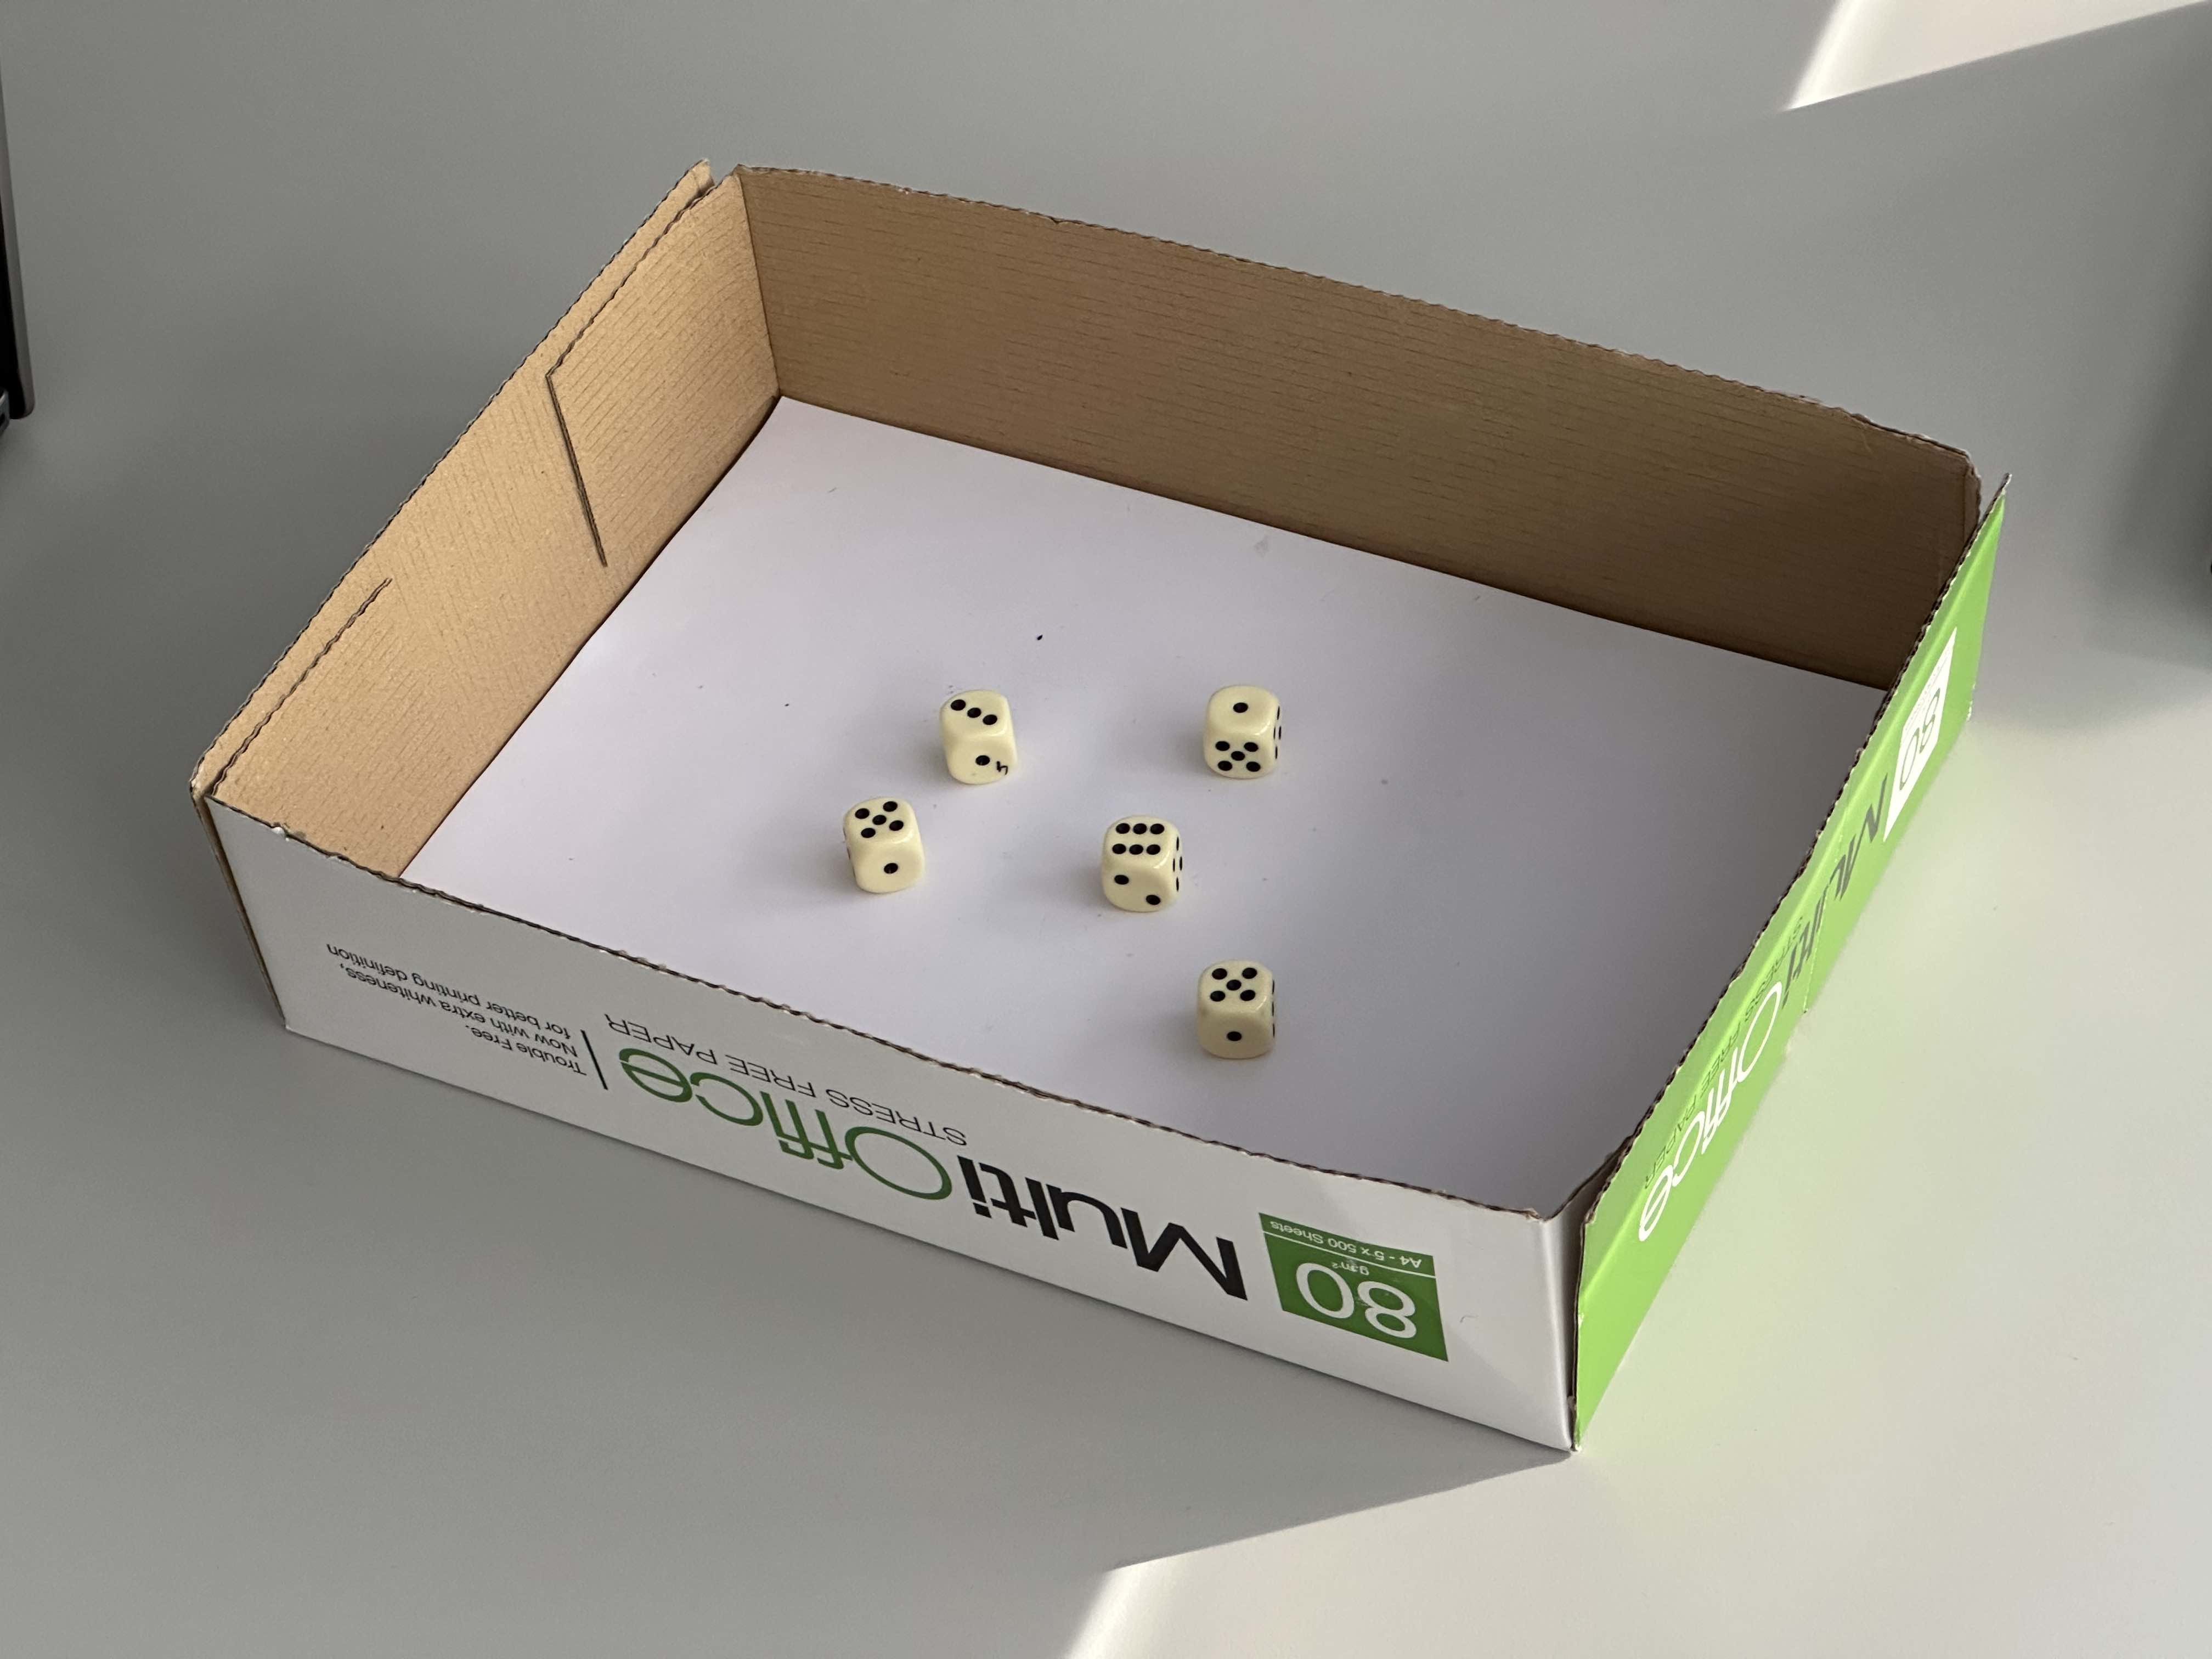
\includegraphics[width=0.5\textwidth]{bilder/Versuchsaufbau1.jpg}           %// [ ] TODO: Versuchsaufbau Bild anpassen
    \caption{<>}                                                                %// [ ] TODO: Versuchsaufbau Bildunterschrift anpassen
    \label{AbbVersuchsaufbau1}
\end{figure}

\subsection{Durchführung}
%//[ ] TODO: Durchführung
% Wie wurde der Versuch durchgeführt bzw. ausgewertet?
% auch wann und wo?

<>

\section{Messergebnisse und Auswertung}
%//[ ] TODO: Messung - evtl. nur Verweis auf Messergebnisse
% Eigentliche Messung!
% Wie groß sind die Messunsicherheiten („Messfehler“)?

Die Messwerte sind dem auf \url{https://eln.jku.at/} zugänglichen bzw. angehängten Laborprotokoll \glqq <>\grqq{} zu entnehmen.         %//[ ] TODO: Protokoll Dateiname anpassen

%//[ ] TODO: Auswertung
% evtl. Formeln, etc.
% auf richtiges Runden der Werte achten
% evtl. auf Gleichungen Bezug nehmen

\begin{equation}
    \label{Gl1}
    x = x
\end{equation}

\vspace{0,5cm}


% Diagramm(e) der Auswertung
\begin{figure}[H]
    \label{AbbAuswertung1}
    \centering
    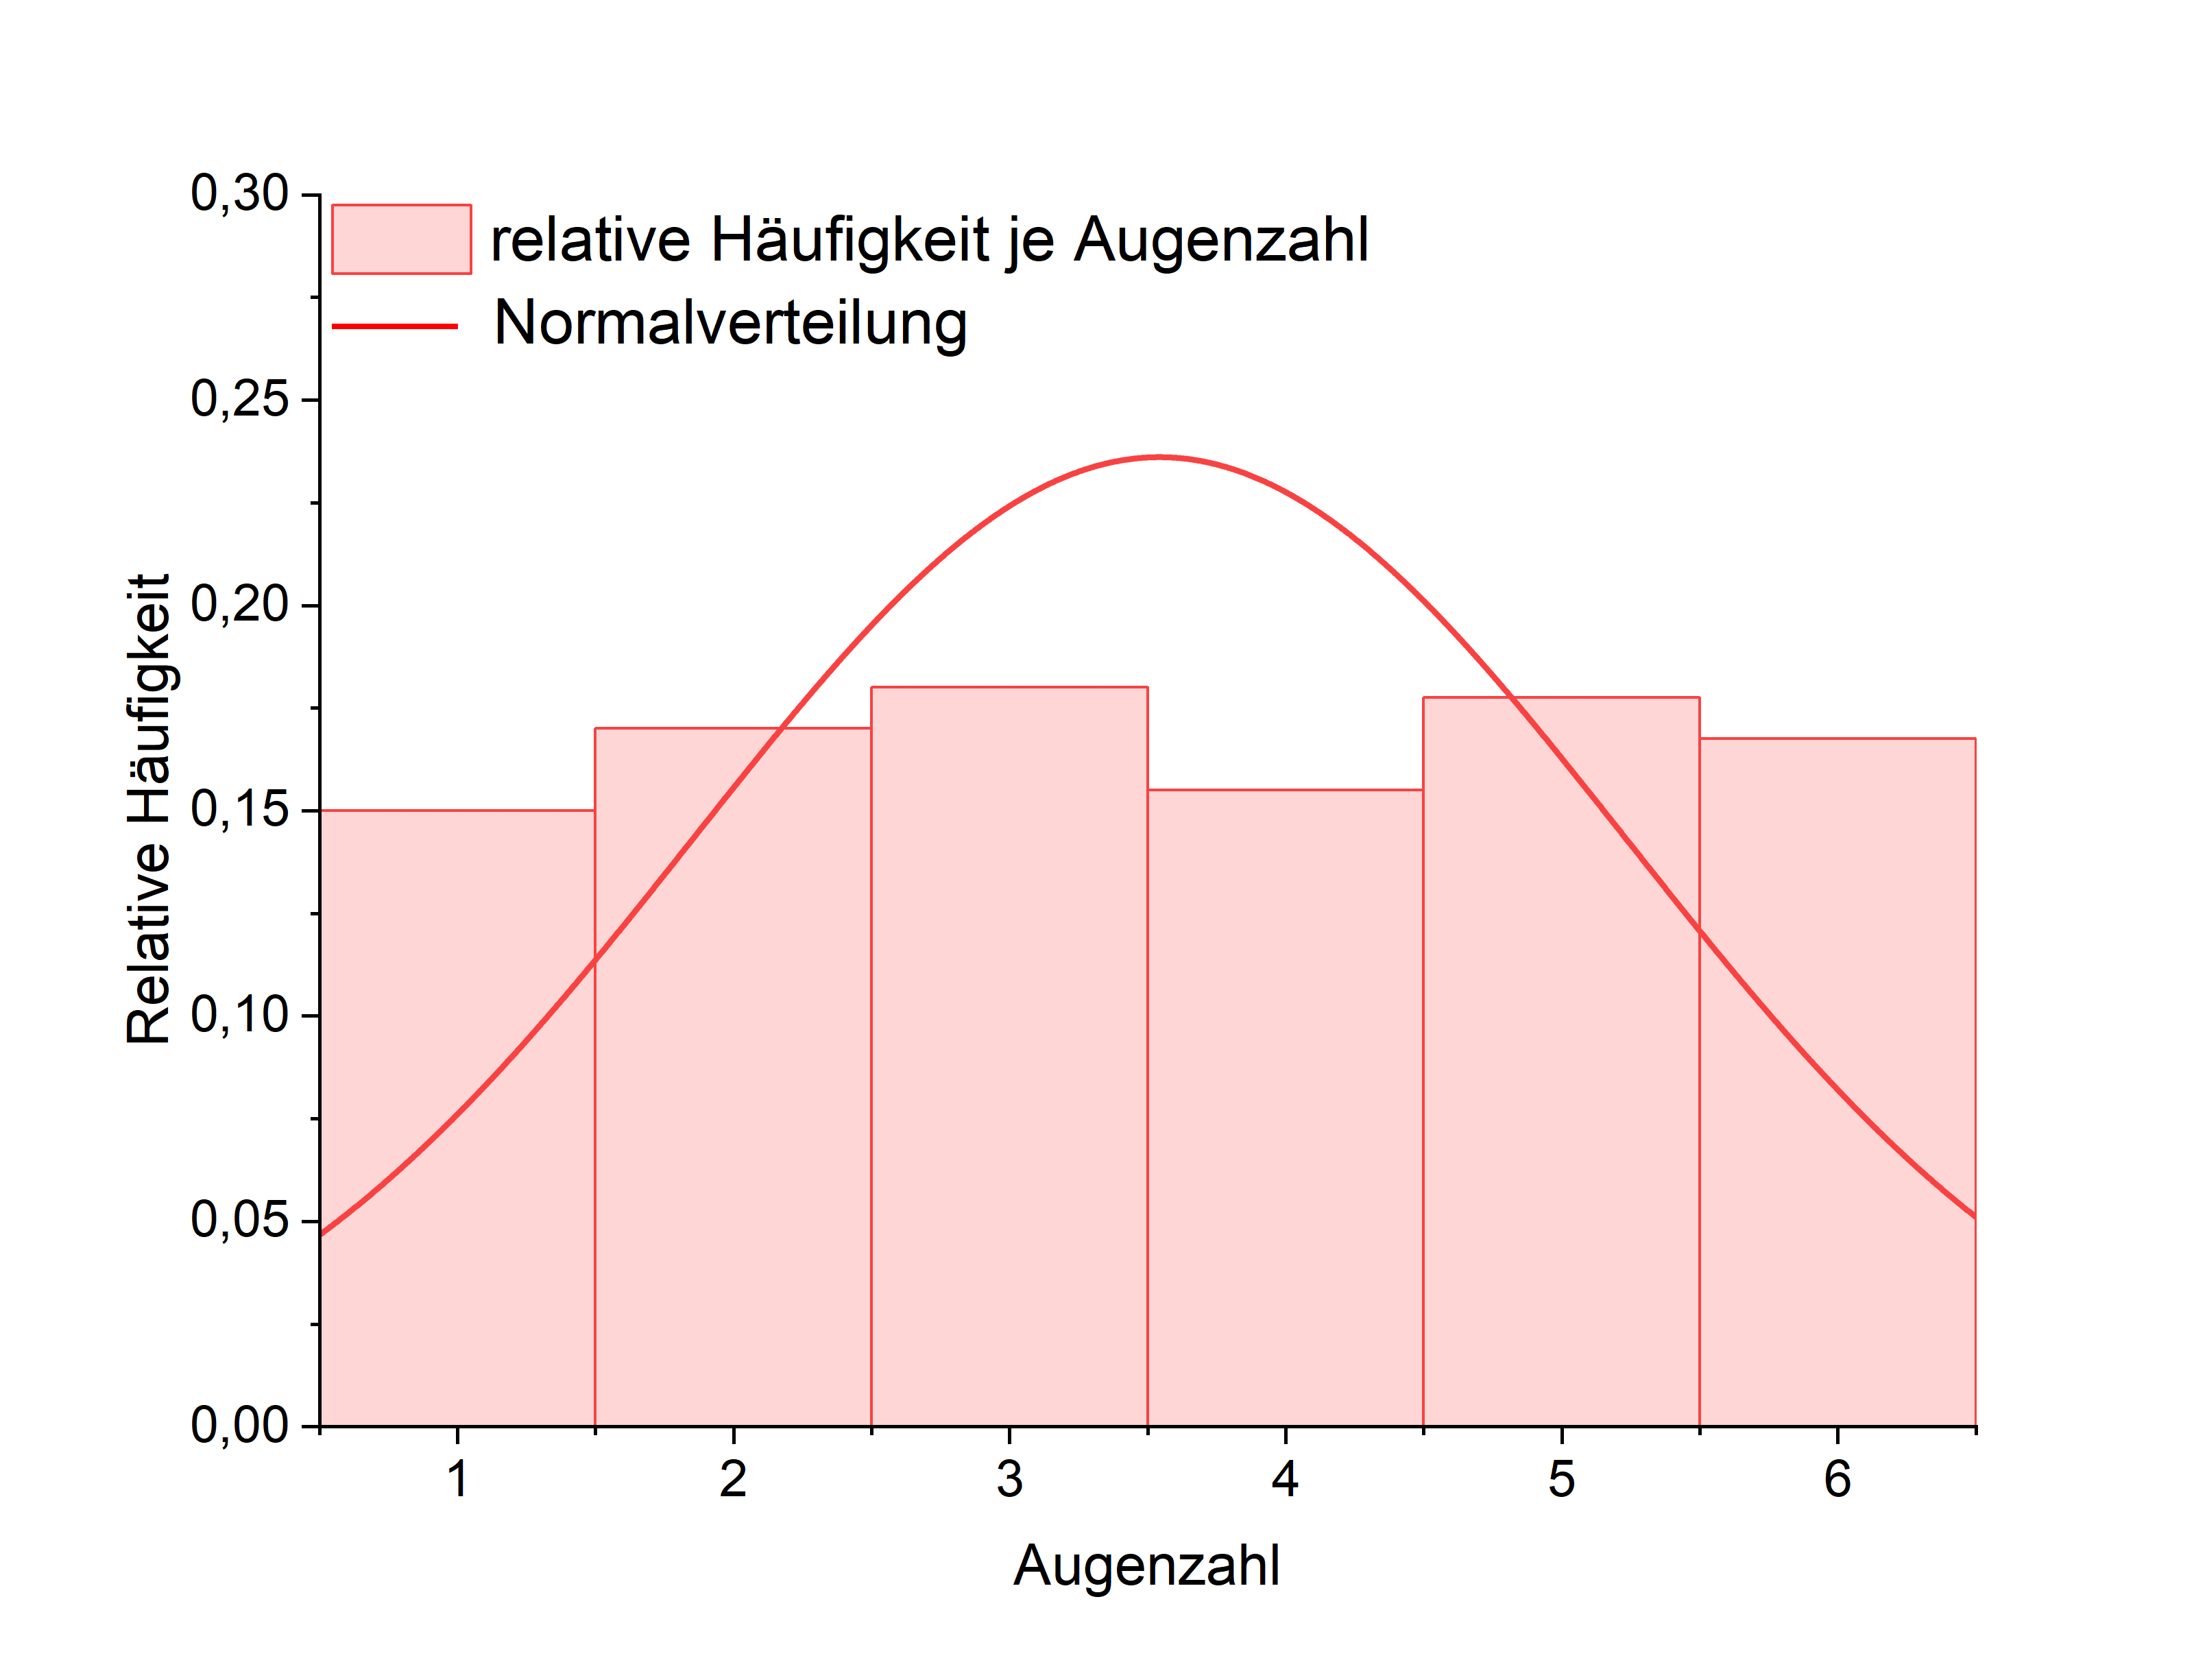
\includegraphics[width=\textwidth]{bilder/Diagramm1.png}        %// [ ] TODO: Diagramm Bild anpassen
    \caption{<>}                                                    %// [ ] TODO: Diagramm Bildunterschrift anpassen
\end{figure}

\section{Diskussion}
%//[ ] TODO: Diskussion
% Wie vergleicht sich meine Messung mit anderen Messungen/Theorien?
% Ist der Messwert sinnvoll? Stimmt die Größenordnung?
% Wo wurden Fehler gemacht? Was kann man verbessern?
% Gegebenenfalls rekursiv auswerten oder nachmessen!
% ursprüngliche Fragestellung diskutieren
% zB Standardabweichung diskutieren, berechnete Größen nennen

<>

\end{document}
